\hfill \newline
\textbf{Analysis\#1} \newline
\phantom{ } We first built three circuits with the same schematic shown in figure[\ref{fig:circ1}] with the power supply $\pm12\si{\volt}$ to the amplifier but of different capacitors, where $R_1=R_2=240\si{\kilo\ohm},R_3=R_4=2.4\si{\kilo\ohm}$, and the left-to-right resistance of $R_5$ is $100\si{\kilo\ohm}$. According to the prelab result, we had the following values for capacitors, shown in table[\ref{tab:chos}].

\begin{figure}[!htbp]
	\centering
	\begin{framed}
		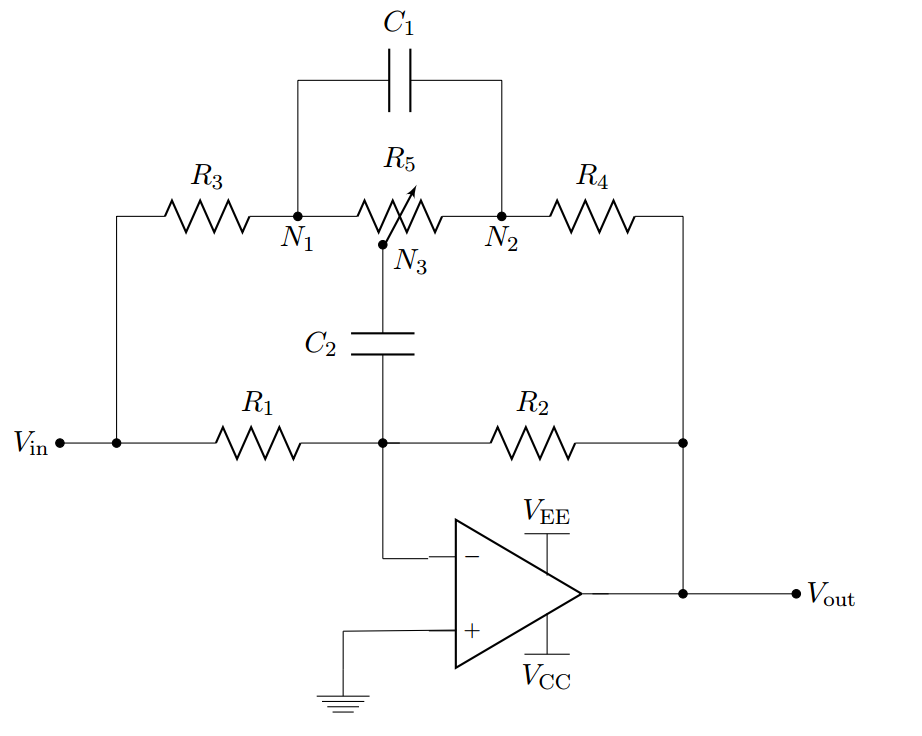
\includegraphics[width=\linewidth]{images/circ1.png}
		\caption{The equalizer filter schematic}
		\label{fig:circ1}
	\end{framed}
\end{figure}

\begin{table}[!htbp]
	\centering
	\caption{Capacitance of capacitors in the filters}
	\begin{tabular}{lcc}
		\toprule
		center frequency & $C_1$ & $C_2$ \\
		\midrule
		$250\si{\hertz}$ & $0.1\si{\micro\farad}$ & $0.0047\si{\micro\farad}$ \\
		$1\si{\kilo\hertz}$ & $0.022\si{\micro\farad}$ & $0.0022\si{\micro\farad}$ \\
		$4\si{\kilo\hertz}$ & $0.0056\si{\micro\farad}$ & $560\si{\pico\farad}$ \\
		\bottomrule
	\end{tabular}
	\label{tab:chos}
\end{table}

To make sure that those circuits works well as band-pass. We measured the frequency response of the gain of each circuit, in the 1-2-5 method, from $10\si{\hertz}$ to $5\si{\kilo\hertz}$. The results are displayed in table[\ref{tab:data00},\ref{tab:data01},\ref{tab:data02},\ref{tab:data10},\ref{tab:data11},\ref{tab:data12},\ref{tab:data20},\ref{tab:data21},tab:data22}]

\begin{table}[!htbp]
	\centering
	\caption{$Measurments of 25\%$ - $250\si{\hertz}$}
	\label{tab:data00}
	\begin{tabular}{lccc}
		\toprule
		frequency($\si{\hertz}$) & $V_{in}$($\si{\milli\volt}$) & $V_{out}$($\si{\milli\volt}$) & gain($\si{\decibel}$) \\
		\midrule
		10	&224&	232&	0.305\\
		20	&232&	236&	0.148\\
		50	&232&	252&	0.718\\
		100	&224&	280&	1.938\\
		200	&220&	356&	4.181\\
		500	&220&	368&	4.469\\
		1000&	244&	280&	1.195\\
		2000&	232&	248&	0.579\\
		5000&	232&	244&	0.438\\
		10000&	232&	240&	0.294\\
		20000&	240&	224&	-0.599\\
		50000&	232&	228&	-0.151\\
		\bottomrule
	\end{tabular}
\end{table}

\begin{table}[!htbp]
	\centering
	\caption{$Measurments of 25\%$ - $1\si{\kilo\hertz}$}
	\label{tab:data01}
	\begin{tabular}{lccc}
		\toprule
		frequency($\si{\hertz}$) & $V_{in}$($\si{\milli\volt}$) & $V_{out}$($\si{\milli\volt}$) & gain($\si{\decibel}$) \\
		\midrule
		10&	224&	232&	0.305\\
		20&	228&	228&	0.000\\
		50&	220&	224&	0.157\\
		100&	224&	236&	0.453\\
		200&	220&	268&	1.714\\
		500&	220&	384&	4.838\\
		1000&	224&	428&	5.624\\
		2000&	228&	324&	3.052\\
		5000&	228&	246&	0.660\\
		10000&	232&	232&	0.000\\
		20000&	236&	236&	0.000\\
		50000&	232&	240&	0.294\\
		\bottomrule
	\end{tabular}
\end{table}

\begin{table}[!htbp]
	\centering
	\caption{$Measurments of 25\%$ - $1\si{\kilo\hertz}$}
	\label{tab:data01}
	\begin{tabular}{lccc}
		\toprule
		frequency($\si{\hertz}$) & $V_{in}$($\si{\milli\volt}$) & $V_{out}$($\si{\milli\volt}$) & gain($\si{\decibel}$) \\
		\midrule
		10&	224&	232&	0.305\\
		20&	228&	228&	0.000\\
		50&	220&	224&	0.157\\
		100&	224&	236&	0.453\\
		200&	220&	268&	1.714\\
		500&	220&	384&	4.838\\
		1000&	224&	428&	5.624\\
		2000&	228&	324&	3.052\\
		5000&	228&	246&	0.660\\
		10000&	232&	232&	0.000\\
		20000&	236&	236&	0.000\\
		50000&	232&	240&	0.294\\
		\bottomrule
	\end{tabular}
\end{table}